% !TEX program = xelatex
\documentclass[a4paper]{article}
\usepackage{amsthm}
\usepackage{amssymb}
\usepackage{bm}
\usepackage{mathtools}
\usepackage[x11names]{xcolor}
\usepackage{xparse}
\usepackage{fontspec}
\usepackage{unicode-math}
\setromanfont[Ligatures={Common,Rare}]{DovesType-Regular.otf}
\setsansfont{Andika}
\setmathfont{Asana Math}[Scale=1]
\newfontfamily\TrajanP[Scale=1.0]{TRAJANPRO-REGULAR.OTF}
% \newfontfamily\TrajanP[Scale=1.0]{Tork}

% \usepackage{pstricks}
\usepackage{varwidth}
\usepackage{siunitx}
\usepackage{graphicx}
\usepackage[margin=1.5cm,top=1.5cm]{geometry}
\usepackage[most]{tcolorbox}
\usepackage{pgfplots}
\pgfplotsset{compat=newest}
\tcbuselibrary{skins,xparse,poster,breakable}
% \usetikzlibrary{fadings}
\usetikzlibrary{calc,math, plotmarks, shapes, shapes.geometric, positioning, angles, intersections, quotes, through, patterns, turtle, arrows.meta}
\usetikzlibrary{decorations.markings,backgrounds}
% \usepackage{etoolbox}
\usepackage{tkz-euclide}
% \usepackage{xlop}
% \newcommand\hole[2]{#1}  % for use with xlop
\pagenumbering{gobble}
%%%%%%%%%%%%%%%%%%%%%%%%%%%%%%%%%%%%%%%%%%%%%%%%%%%%%%%%%
\newcommand\markangle[9]{% origin X Y radius radiusmark mark colour opacity
%  % fill red circle offset-from-centre
  \begin{scope}
    \path[clip] (#1) -- (#2) -- (#3);
    \fill[color=#7,fill opacity=#8,draw=black,name path global=pcircle]  % global declaration required otherwise pcircle is not seen by the `named intersections=' lines below.
    (#1) circle (#4);
  \end{scope}
  % middle calculation
  \path[name path=line one] (#1) -- (#2);
  \path[name path=line two] (#1) -- (#3);
  \path[%
  name intersections={of=line one and pcircle, by={inter one}},
  name intersections={of=line two and pcircle, by={inter two}}
  ] (inter one) -- (inter two) coordinate[pos=#9] (place);
  % put mark
  \node at ($(#1)!#5!(place)$) {\scriptsize{#6}};
}
%%%%%%%%%%%%%%%%%%%%%%%%%%%%%%%%%%%%%%%%%%%%%%%%%%%%%%%%
\newcommand\tcircle[6]{% centre coord (x,y), radius, points, radpoint, colour, edge
  \coordinate (O) at (#1,#2); % centre of the circle
  \def\radius{#3}          % radius of the circle
  \def\npts{#4}            % number of the points
  \def\radpt{#5}           % radius of the points
  \colorlet{ptcolour}{#6}  % colour of the points
  % \draw (O) circle (\radius);
  \foreach \numpoint in {1,...,\npts}{
    \fill[ptcolour] (O) ++ (360/\npts*\numpoint:\radius) coordinate (C\numpoint) circle(\radpt);
  }
}

% \newcommand{\condSoln}[2]{\ifcsdef{r@#1}{#2}{}}

% \newcommand\fadingtext[3][]{%
%    \begin{tikzfadingfrompicture}[name=fading letter]
%      \node[text=transparent!0,inner xsep=0pt,outer xsep=0pt,#1] {#3};
%    \end{tikzfadingfrompicture}%
%    \begin{tikzpicture}[baseline=(textnode.base)]
%      \node[inner sep=0pt,outer sep=0pt,#1](textnode){\phantom{#3}};
%      \shade[path fading=fading letter,#2,fit fading=false]
%      (textnode.south west) rectangle (textnode.north east);%
%    \end{tikzpicture}%
% }

\definecolor{JISpurple}{RGB}{89,72,122}
\definecolor{JISivory}{RGB}{241,234,221}
\definecolor{JIStaupe}{RGB}{183,156,154}
\definecolor{PaleGreen}{RGB}{240,255,240} % 'Honeydew'

\AddToHook{shipout/background}{%
    \put (0in,-\paperheight){\includegraphics[width=\paperwidth,height=\paperheight]{images/penrose2r.jpg}}%
}

\newcommand\numberthis{\addtocounter{equation}{1}\tag{\theequation}}

\newtcolorbox{MyOuterBox}{%
  enhanced,
  % watermark graphics=images/santa_faces_watermark.jpg,
  % watermark opacity=0.8,
  % watermark zoom=2.0,
  breakable,
  frame style=JISpurple,
  colback=JISivory,
  colframe=JISpurple,
  title={\includegraphics[width=0.9cm,height=0.9cm]{images/JIS Final Logo FA-02.png}\raisebox{3mm}{\Large{Maths Challenge}\hspace{24em} \Large{\bfseries\sffamily 19}}},
}

\newtcolorbox{MyInnerBox}[2][]{enhanced,%empty,
coltitle=JISpurple,colback=white,
breakable,
fonttitle=\bfseries\sffamily,
attach boxed title to top left={yshift=-1.5mm},
boxed title style={empty, size=small, top=1mm, bottom=0pt},
varwidth boxed title=0.5\linewidth,
frame code={
  \path (title.east|-frame.north) coordinate (aux);
\path[draw=JISpurple, line width=0.5mm, rounded corners,fill=white]
(frame.west) |- ([xshift=-2.5mm]title.north east) to[out=0, in=180] ([xshift=7.5mm]aux)-|(frame.east)|-(frame.south)-|cycle;
},
title={#2},#1}

\newtcolorbox{MyInnerSplitBox}[2][]{enhanced,%empty,
bicolor,sidebyside,sidebyside align=top seam,
righthand width=7.5cm,colbacklower=white,
sidebyside gap=5mm,
breakable,
coltitle=JISpurple,colback=white,
fonttitle=\bfseries\sffamily,
attach boxed title to top left={yshift=-1.5mm},
boxed title style={empty, size=small, top=1mm, bottom=0pt},
varwidth boxed title=0.5\linewidth,
frame code={
  \path (title.east|-frame.north) coordinate (aux);
\path[draw=JISpurple, line width=0.5mm, rounded corners,fill=white]
(frame.west) |- ([xshift=-2.5mm]title.north east) to[out=0, in=180] ([xshift=7.5mm]aux)-|(frame.east)|-(frame.south)-|cycle;
},
title={#2},#1}


\newtcolorbox{MySolutionBox}[1][]{%
  enhanced,
  breakable,
  frame style=JISpurple,
  colback=PaleGreen, colframe=green,
  title={\Large Solution},
  drop fuzzy shadow,
  halign=left,
  #1
}

%%%%%%%%%%%%%%%%%%%%%%%%%%%%%%%%%%%%%%%%%%%%%%%%%%
\newtoggle{SOLUTION}
%%% Uncomment the appropriate line below to show solutions %%%
% \toggletrue{SOLUTION}
\togglefalse{SOLUTION}
%%%%%%%%%%%%%%%%%%%%%%%%%%%%%%%%%%%%%%%%%%%%%%%%%


%%%%%%%%%%%%%%%%%%%%%%%%%%%%%%%%%%%%%%%%%%%%%%%%%%
%%%%%%            DOCUMENT BEGINS           %%%%%%
%%%%%%%%%%%%%%%%%%%%%%%%%%%%%%%%%%%%%%%%%%%%%%%%%%
\begin{document}


  \begin{MyOuterBox}
    \iftoggle{SOLUTION}{Here are the full, or partial solutions.
    }{
      Welcome to this week's Maths Challenge!\\
      Have a go at both questions!\\
      Drop your solution in the box in the staffroom by Tuesday.
    }
       \begin{MyInnerBox}{Year 8 and below}
     You have two, identical timer-sticks. Each stick takes exactly 60 minutes to burn along its whole length. The sticks burn non-uniformly: for example, one half of the length of a stick might burn in 15 minutes while the other half takes 45 minutes. You have a lighter to ignite the sticks.\par
        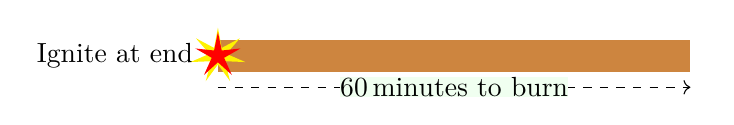
\begin{tikzpicture}[scale=1]
          \draw[line width=4mm,Tan3] (0,2) node[left,black] {Ignite at end}-- (6,2);
          \draw[dashed,->] (0,1.6)  -- (6,1.6) node[midway,inner sep=0mm,fill=PaleGreen] {\(\SI{60}{minutes}\) to burn};
          \node[star,star points=7,star point ratio=-0.7,fill=yellow,minimum width=0.5cm] at (0,2) {};
          \node[star,star points=5,star point ratio=-0.5,fill=red,minimum width=0.3cm] at (0,2) {};
        \end{tikzpicture}\par\medskip
     How can you measure out 45 minutes?\par
      \iftoggle{SOLUTION}{%conditional output begin
      \begin{MySolutionBox}
        If we light one of the sticks at both ends, it will take half the original time, that is, 30 minutes, to burn completely. Notice that this is true even though the rate of burning along the stick is not uniform, this just means that the point where the two burning points meet may not be in the middle of the stick.\par
        So, we light one of the sticks, Stick 1, at both ends, and we light the other stick, Stick 2, at one end.\par\medskip
        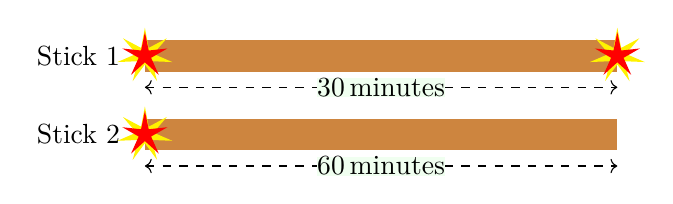
\begin{tikzpicture}[scale=1]
          \draw[line width=4mm,Tan3] (0,3) node[left,black] {Stick 1} -- (6,3);
          \draw[dashed,<->] (0,2.6) -- (6,2.6) node[midway,inner sep=0mm,fill=PaleGreen] {\(\SI{30}{minutes}\)};
          \draw[line width=4mm,Tan3] (0,2) node[left,black] {Stick 2 }-- (6,2);
          \draw[dashed,<->] (0,1.6)  -- (6,1.6) node[midway,inner sep=0mm,fill=PaleGreen] {\(\SI{60}{minutes}\)};
          \node[star,star points=7,star point ratio=-0.7,fill=yellow,minimum width=0.5cm] at (0,3) {};
          \node[star,star points=5,star point ratio=-0.5,fill=red,minimum width=0.3cm] at (0,3) {};
          \node[star,star points=7,star point ratio=-0.7,fill=yellow,minimum width=0.5cm] at (6,3) {};
          \node[star,star points=5,star point ratio=-0.5,fill=red,minimum width=0.3cm] at (6,3) {};
          \node[star,star points=7,star point ratio=-0.7,fill=yellow,minimum width=0.5cm] at (0,2) {};
          \node[star,star points=5,star point ratio=-0.5,fill=red,minimum width=0.3cm] at (0,2) {};
        \end{tikzpicture}\par\medskip
        Thirty minutes later, Stick 1 finishes burning, and thirty minutes burning time is left on Stick 2.\par
        As soon as Stick 1 completes, we light the other end of Stick 2. With one end burning there were thirty minutes left, but with both ends burning, Stick 2 only has \(\SI{15}{\minute}\) of burning time left.\par
        So when Stick 2 is completely burned, \(45\) minutes will have elapsed.\par\medskip
        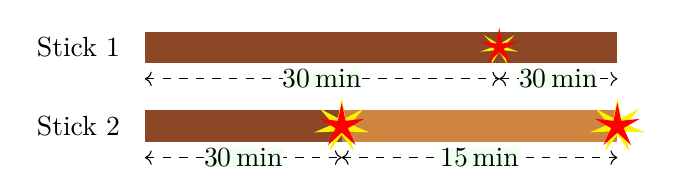
\begin{tikzpicture}[scale=1]
          \draw[line width=4mm,Sienna4] (0,3) node[left,black] {Stick 1} -- (6,3);
          \draw[dashed,<->] (0,2.6) -- (4.5,2.6) node[midway,inner sep=0mm,fill=PaleGreen] {\(\SI{30}{min}\)};
          \draw[dashed,<->] (4.5,2.6) -- (6,2.6) node[midway,inner sep=0mm,fill=PaleGreen] {\(\SI{30}{min}\)};
          \draw[line width=4mm,Sienna4] (0,2) node[left,black] {Stick 2}-- (2.5,2);
          \draw[line width=4mm,Tan3] (2.5,2) -- (6,2);
          \draw[dashed,<->] (0,1.6)  -- (2.5,1.6) node[midway,inner sep=0mm,fill=PaleGreen] {\(\SI{30}{min}\)};
          \draw[dashed,<->] (2.5,1.6)  -- (6,1.6) node[midway,inner sep=0mm,fill=PaleGreen] {\(\SI{15}{min}\)};
          \node[star,star points=7,star point ratio=-0.4,fill=yellow,minimum width=0.2cm] at (4.5,3) {};
          \node[star,star points=5,star point ratio=-0.4,fill=red,minimum width=0.2cm] at (4.5,3) {};
          \node[star,star points=7,star point ratio=-0.7,fill=yellow,minimum width=0.5cm] at (6,2) {};
          \node[star,star points=5,star point ratio=-0.5,fill=red,minimum width=0.3cm] at (6,2) {};
          \node[star,star points=7,star point ratio=-0.7,fill=yellow,minimum width=0.5cm] at (2.5,2) {};
          \node[star,star points=5,star point ratio=-0.5,fill=red,minimum width=0.3cm] at (2.5,2) {};
        \end{tikzpicture}
      \end{MySolutionBox}
    }{}%conditional output end
    \end{MyInnerBox}


    \vspace{0.4cm}
          \begin{MyInnerBox}{Year 9 and above}
        Find the green angle.\par
        \begin{tikzpicture}[scale=1]
          \coordinate (A) at (4,5);
          \coordinate (B) at (0,2);
          \coordinate (C) at (4,0);
          \coordinate (D) at (7,1);
          \draw[decoration={markings,mark=at position 0.5 with {\draw(-1pt,-3pt) -- (1pt,3pt);}},postaction={decorate}] (A) -- (B);
          \draw[decoration={markings,mark=at position 0.5 with {\draw(-1pt,-3pt) -- (1pt,3pt);}},postaction={decorate}] (A) -- (C);
          \draw[decoration={markings,mark=at position 0.5 with {\draw(-1pt,-3pt) -- (1pt,3pt);}},postaction={decorate}] (A) -- (D);
          \draw (B) -- (D) (C) -- (D);
          \markangle{A}{B}{C}{5mm}{7mm}{\(\SI{50}{\degree}\)}{blue!70}{0.7}{0.7}
          \markangle{D}{B}{C}{5mm}{7mm}{}{green!70}{0.7}{0.7}
          \iftoggle{SOLUTION}{
            \node[above] at (A) {\(A\)};
            \node[below left] at (B) {\(B\)};
            \node[below] at (C) {\(C\)};
            \node[below right] at (D) {\(D\)};
            \draw[thick,blue] ([shift=(210:5cm)]A) arc (210:320:5cm);
          }{}
        \end{tikzpicture}
      \iftoggle{SOLUTION}{%conditional output begin
      \begin{MySolutionBox}
        We are told that \(AB=AC=AD\). If we take these three lengths as the radii of a circle centre \(A\), then the arc \(BC\) subtends an angle of \(\SI{50}{\degree}\) at the centre.\par
        We can see that the same arc \(BC\) subtends the green angle at \(D\) on the circumference of the circle.\par
        By the circle theorem: angle at the centre is twice the angle at the circumference (see No. 16), \(\angle BDC = \frac{1}{2}\angle BAC\), so the green angle is \(\SI{25}{\degree}\)\par
      \end{MySolutionBox}
    }{}%conditional output end
    \end{MyInnerBox}


  \end{MyOuterBox}

%%%%%%%%%%%%%%%%%%%%%%%%%%%%%%%%%%%%%%%%%%%%%%%%%%
\end{document}



